\documentclass[11pt]{article}

\usepackage[margin=1in]{geometry}
\usepackage[T1]{fontenc}
\usepackage{amsmath,amssymb}
\usepackage{booktabs}
\usepackage{enumitem}
\usepackage{graphicx}
\usepackage{caption}
\usepackage{xcolor}
\usepackage{tikz}
\usetikzlibrary{arrows.meta,positioning,fit}
\usepackage{hyperref}

\hypersetup{
  colorlinks=true,
  linkcolor=blue!60!black,
  citecolor=blue!60!black,
  urlcolor=blue!60!black
}

\setlist[itemize]{leftmargin=1.5em}
\setlist[enumerate]{leftmargin=1.7em}

\newcommand{\code}[1]{\texttt{#1}}

\title{Full-Waveform Inversion for Ring-Array Ultrasound:\\
Algorithm, Simulation Setup, and Abdominal CT Results}
\author{Sarang Joshi}
\date{\today}

\begin{document}

\maketitle

\begin{abstract}
This note describes the time-domain full-waveform inversion (FWI) implemented in
\code{invert\_ring.py}, which recovers a two-dimensional sound-speed map from
ring-array ultrasound traces, and \code{totalseg\_to\_speed.py}, which builds
abdominal sound-speed maps from an open, expert-segmented CT dataset and a
table of tissue acoustic properties. On a TotalSegmentator abdomen
(1450--3750~m/s, 128 elements, three frequency stages) the misfit falls in
every stage, but the bone is not recovered: the vertebral body comes out
hollow, the ribs are missing and false bone-speed patches appear, so the
interior RMS error (314.7~m/s) ends slightly above that of the starting model
(293.1~m/s). An earlier run on a threshold-based KiTS-00136 abdomen showed the
same bone failure while recovering soft-tissue anatomy. Both point to cycle
skipping in bone as the main obstacle.
\end{abstract}

\section{Forward model}

The forward model is the 2D constant-density acoustic wave equation,
discretized with second-order finite differences in space and time (FDTD).
Sound speed $c(\mathbf{x})$ is the only material property; density and
attenuation are constant:
\begin{equation}
  \frac{\partial^2 u}{\partial t^2} = c(\mathbf{x})^2\,\nabla^2 u
  + s(t)\,\delta(\mathbf{x}-\mathbf{x}_{\mathrm{tx}}).
\end{equation}

\begin{itemize}
  \item \textbf{Time stepping.} A leapfrog scheme advances the pressure,
    $u^{n+1} = 2u^n - u^{n-1} + \Delta t^2 c^2 L[u^n]$, where $L$ is the
    5-point Laplacian applied as a $3\times3$ convolution.
  \item \textbf{Stability.} The step obeys the 2D CFL bound
    $c_{\max}\,\Delta t\,\sqrt{1/\Delta x^2 + 1/\Delta y^2} < 1$. The code uses a
    CFL number of 0.45, with $c_{\max}$ the larger of the true medium maximum
    and the upper reconstruction bound.
  \item \textbf{Boundaries.} First-order Mur absorbing conditions on all four
    edges; corners average the $x$- and $y$-direction updates.
  \item \textbf{Sources and receivers.} A transmitter is a soft (additive) point
    source at its nearest grid node. Receivers sample pressure by bilinear
    interpolation, so element positions are not locked to pixel centres.
  \item \textbf{Execution.} Fields stay on one PyTorch device (CPU, CUDA or
    Apple MPS). Independent transmitter shots are advanced together as a batch,
    and on CUDA the step is compiled with \code{torch.compile}.
\end{itemize}

\section{Simulation setup}
\label{sec:setup}

A ring of point transducers surrounds the object; each element both transmits
and receives. One element fires a chirp per shot and every element records,
giving an $N \times N \times$ time dataset. Two configurations are used: the
default phantom setup (200~mm field of view, 70~mm ring) and the abdominal
setup, which scales the grid and ring to fit a 0.3~m-wide torso.

\subsection{Acquisition and discretization}

\begin{table}[ht]
\centering
\small
\caption{Simulation parameters. Abdomen values (TotalSegmentator subject
  s1366) are listed per multiscale stage.}
\label{tab:setup}
\begin{tabular}{@{}lll@{}}
\toprule
Parameter & Phantom setup (default) & Abdomen setup, per stage \\
\midrule
Grid (cells) & $401 \times 401$ & $101^2 \to 201^2 \to 401^2$ \\
Grid spacing $\Delta x$ & 0.50~mm & 4.00 $\to$ 1.83 $\to$ 1.50~mm \\
Field of view & 200~mm & 404 $\to$ 367 $\to$ 602~mm \\
Ring radius & 70~mm & 167.7 $\to$ 168.3 $\to$ 168.5~mm \\
Elements & 256 (pitch 1.7~mm) & 128 (pitch 8.3~mm) \\
Coupling medium & water, 1500~m/s & water, 1480~m/s \\
Source pulse & Hann-windowed linear chirp, & 25--75~kHz / 80~$\mu$s $\to$ \\
 & 100--250~kHz, 20~$\mu$s & 50--125~kHz / 40~$\mu$s $\to$ 100--250~kHz / 20~$\mu$s \\
Time step $\Delta t$ (CFL 0.45) & $\approx 80$~ns & 326 $\to$ 149 $\to$ 122~ns \\
Record length & $1.6\times$ ring diameter / slowest speed & $\approx 371~\mu$s (1135 $\to$ 2490 $\to$ 3039 steps) \\
Points per shortest wavelength & $\approx 12$ & $\approx$ 4.8 $\to$ 6.3 $\to$ 3.9 \\
Inversion bounds on $c$ & 1400--2000~m/s & 1400--3900~m/s \\
\bottomrule
\end{tabular}
\end{table}

The abdomen time steps follow from the 3900~m/s upper bound, which sets the CFL
limit. The record length is 1.6 times the time to cross the ring diameter at the
slowest speed in the medium (fat, 1450~m/s). The grid is never finer than the CT
pixels, so the final stage runs at the 1.5~mm CT spacing on a 602~mm field of
view, most of it coupling water.

\subsection{Abdominal sound-speed model from an open segmentation}
\label{sec:totalseg}

The medium is one axial slice of a public, expert-segmented CT, converted by
\code{totalseg\_to\_speed.py}. Organs, vessels, bowel, bone and the deep back
muscles come from the segmentation; only pixels no mask covers are classified
by Hounsfield units (HU).

\begin{enumerate}
  \item \textbf{Data.} The \emph{Small subset of TotalSegmentator Dataset}
    v2.0.1 \cite{totalseg_data, wasserthal2023} holds 102 CT volumes resampled to
    1.5~mm, each with masks of 117 structures (CC BY 4.0). \code{--fetch}
    downloads a single subject out of the 3.2~GB zip with HTTP range requests
    (44~MB for subject s1366).
  \item \textbf{Subject choice.} Of the 54 subjects whose masks include the
    main upper-abdominal organs, the cleanest were screened by compressed bytes per voxel,
    then by the HU standard deviation inside the liver after removing a
    $5^3$-voxel local mean. Subject s1366 has 14.7~HU of noise, against 140~HU
    for the noisiest (low-dose) scan, s0407, which was rejected.
  \item \textbf{Slice choice.} Among slices showing all ten key structures
    (liver, spleen, both kidneys, pancreas, stomach, aorta, inferior vena cava,
    both deep back muscles), the one with the least gas inside the body is
    used: slice 259, at the T12/L1 level, with 2.5\% gas.
  \item \textbf{Tissue classes.} Masks are merged into the classes of
    Table~\ref{tab:tissues}. Unlabelled body pixels are classified by HU after
    a $5\times5$ median filter: fat ($-190$ to $-30$), gas ($<-190$) or other
    soft tissue. Gas, which the scalar fluid model cannot represent, becomes
    water; inside segmented solid organs low HU is treated as noise, not gas.
    The body is the largest connected region above $-500$~HU, which excludes
    the arms and the scanner table.
  \item \textbf{Acoustic properties per class.} Each class points to one row
    of \code{abdominal\_acoustic\_parameters.csv} (Table~\ref{tab:acoustic}),
    compiled from \cite{duck1990, szabo, mast2000}. The script writes speed,
    density, power-law attenuation and $B/A$ maps; the present solvers are
    lossless and constant-density, so only speed enters them. Gas is modelled
    as water rather than 343~m/s air: without a density contrast the scalar
    model cannot reproduce the near-total reflection at a gas boundary.
  \item \textbf{Embedding.} \code{load\_ct\_ring\_grid} centres the body,
    resamples it to each stage's grid with nearest-neighbour sampling, pads the
    outside with 1480~m/s water, and places the ring 10~mm outside the body
    with an 8-cell margin to the grid edge.
\end{enumerate}

\begin{table}[ht]
\centering
\small
\caption{Tissue acoustic properties (\code{abdominal\_acoustic\_parameters.csv};
  values compiled from \cite{duck1990, szabo, mast2000}). Attenuation follows
  $\alpha = \alpha_0 f^{\,y}$ with $f$ in MHz.}
\label{tab:acoustic}
\begin{tabular}{@{}lrrrrr@{}}
\toprule
Tissue & $c$ (m/s) & $\rho$ (kg/m$^3$) & $\alpha_0$ (dB/MHz$^y$/cm) & $y$ & $B/A$ \\
\midrule
Soft tissue (machine average) & 1540 & 1000 & 0.5 & 1.1 & 7.0 \\
Water / bile / urine & 1480 & 1000 & 0.0022 & 2.0 & 5.0 \\
Fat (visceral/subcutaneous) & 1450 & 920 & 0.75 & 1.25 & 10.0 \\
Liver & 1570 & 1060 & 0.6 & 1.2 & 6.8 \\
Kidney & 1560 & 1050 & 0.9 & 1.0 & 7.2 \\
Blood & 1575 & 1050 & 0.15 & 1.3 & 6.1 \\
Muscle (abdominal wall) & 1580 & 1080 & 1.1 & 1.0 & 7.4 \\
Spleen & 1567 & 1054 & 0.55 & 1.2 & 6.8 \\
Bowel gas / air & 343 & 1.2 & 12.0 & 2.0 & 0.4 \\
Bone / cortical rib & 3750 & 1900 & 15.0 & 1.5 & 0.0 \\
\bottomrule
\end{tabular}
\end{table}

\begin{table}[ht]
\centering
\small
\caption{Tissue classes of the s1366 slice (333 $\times$ 333 pixels at 1.5~mm)
  and the table row each uses.}
\label{tab:tissues}
\begin{tabular}{@{}lllrr@{}}
\toprule
Class & Source & Property row & $c$ (m/s) & Share of body \\
\midrule
Fat & HU & Fat & 1450 & 31.9\% \\
Other soft tissue & HU & Soft tissue average & 1540 & 23.5\% \\
Liver & mask & Liver & 1570 & 21.8\% \\
Digestive tract (stomach, small bowel, colon) & masks & Soft tissue average & 1540 & 7.1\% \\
Muscle (deep back muscles) & masks & Muscle & 1580 & 4.3\% \\
Gas, modelled as water & HU & Water & 1480 & 2.5\% \\
Bone (T11--L1 vertebrae, ribs) & masks & Bone & 3750 & 2.3\% \\
Kidney & masks & Kidney & 1560 & 2.1\% \\
Blood vessels (aorta, IVC, portal/splenic vein) & masks & Blood & 1575 & 1.9\% \\
Other organs (pancreas, adrenals) & masks & Soft tissue average & 1540 & 1.8\% \\
Spleen & mask & Spleen & 1567 & 0.8\% \\
\bottomrule
\end{tabular}
\end{table}

\begin{figure}[ht]
  \centering
  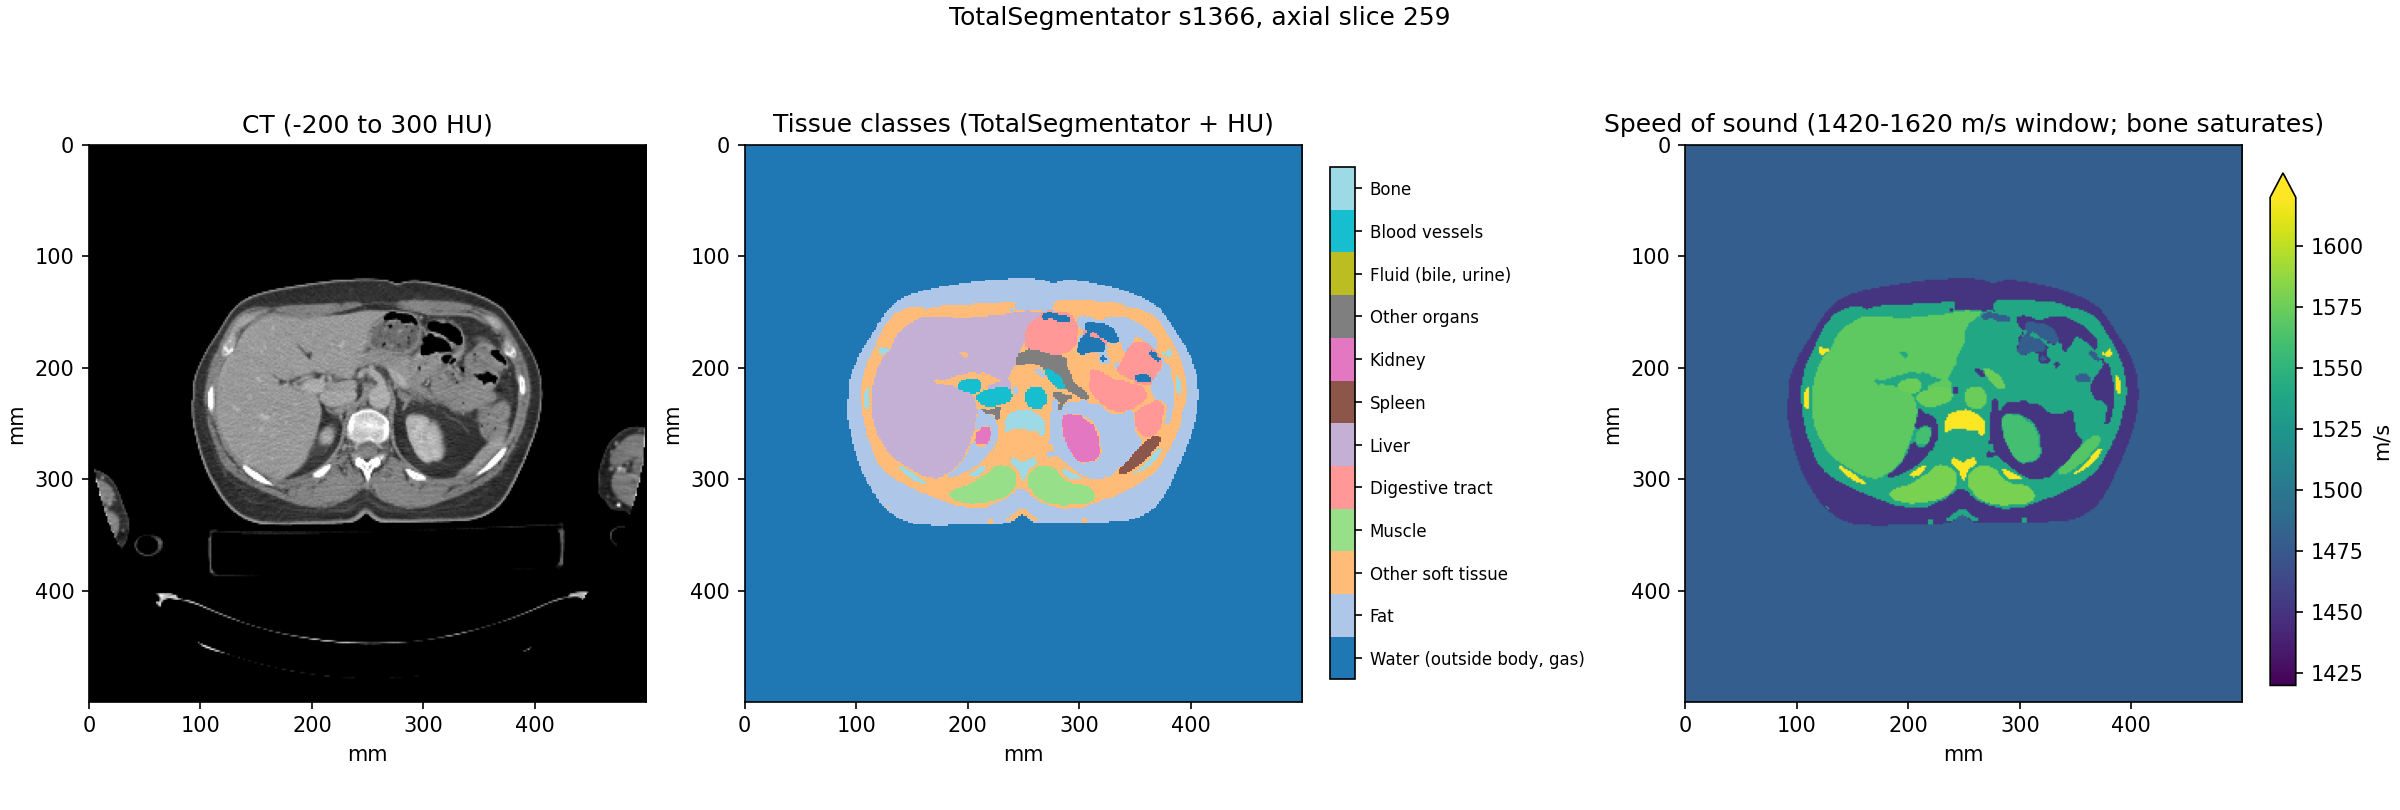
\includegraphics[width=\textwidth]{totalseg_s1366_acoustic.png}
  \caption{TotalSegmentator subject s1366, axial slice 259: CT (window $-200$
    to 300~HU), merged tissue classes, and the resulting sound-speed map. The
    speed map is shown in a 1420--1620~m/s soft-tissue window; bone
    (3750~m/s) saturates at the top of the scale.}
  \label{fig:ct}
\end{figure}

The map spans 1450--3750~m/s. Soft-tissue contrasts are small (within 7\% of
water), while bone is 2.5 times faster than water: it dominates both the data
and the difficulty of the inversion.

\paragraph{Earlier model.} The first experiments
(Section~\ref{sec:kits}) used \code{ct\_to\_speed.py} on one slice of
C4KC-KiTS case KiTS-00136 (512 $\times$ 512 at 0.684~mm). That pipeline has no
anatomical labels: it thresholds HU into air, fat, soft tissue and bone, and
splits superficial from deep tissue at 25~mm depth (fat into subcutaneous and
visceral, soft tissue into muscle and organs), with representative speeds from
Table~1 of \cite{culjat2010} (1478--3476~m/s). The segmentation-based model
replaces that depth rule with real organ, vessel and muscle boundaries.

\section{Inversion algorithm}
\label{sec:algorithm}

The inversion minimizes the least-squares misfit between simulated and observed
traces over slowness squared $m = 1/c^2$, using an exact discrete adjoint for
the gradient and first-order updates. Everything below is implemented in
\code{invert\_ring.py} and \code{fdtd2d/inversion/}.

\subsection{Unknowns and constraints}

\begin{itemize}
  \item \textbf{Parameter.} $m = 1/c^2$ on every pixel inside an interior disk
    $\Omega$ of radius (ring radius $-$ margin), with a 2-pixel margin by
    default. Outside $\Omega$, $c$ is fixed at the coupling-medium speed. The
    wave operator is linear in $c^2 = 1/m$, which keeps the gradient simple.
  \item \textbf{Bounds.} After every update $m$ is projected onto
    $[1/c_{\max}^2,\, 1/c_{\min}^2]$ and the exterior is reset to the
    background.
  \item \textbf{Starting model.} Homogeneous coupling medium (1500 or
    1480~m/s) inside the mask.
\end{itemize}

\subsection{Objective}

\begin{equation}
  J(m) = \frac{1}{2}\sum_{s \in S}\sum_{r \neq s}\sum_{n}
  \left(d^{\,\mathrm{pred}}_{s,r,n}(m) - d^{\,\mathrm{obs}}_{s,r,n}\right)^2
  + \frac{\alpha}{2}\,\lVert \nabla m \rVert^2_{\Omega}.
\end{equation}
$S$ is the set of active transmitters, $r$ runs over receivers and $n$ over
time samples. The transmitter's own channel is excluded because a point
source's direct pressure is a poorly conditioned datum. The Tikhonov term
penalizes differences between neighbouring pixels inside $\Omega$; its weight
$\alpha$ (\code{-{}-reg}) defaults to 0.

Observed data are synthetic: at the start of each stage the same solver
simulates all $N$ transmitters through the true medium, without noise.

\subsection{Adjoint-state gradient}

For each active shot the forward pass stores the full wavefield history $u^n$.
The adjoint field $\lambda$ is then stepped backward in time with the transposed
operator $L(c^2\,\cdot)$, driven by the residuals scattered onto the grid by
the transpose of the bilinear receiver sampling. The gradient with respect to
$c^2$ accumulates as
\begin{equation}
  g_{c^2} = \Delta t^2 \sum_{n} \lambda^{n} \odot L\!\left[u^{\,n-1}\right],
  \qquad
  \frac{\partial J}{\partial m} = -\frac{g_{c^2}}{m^2} + \alpha\,\nabla_m R(m).
\end{equation}
The gradient is set to zero outside the mask. The adjoint reuses the forward Mur
boundary update, which is not its exact transpose; the finite-difference
gradient check (Section~\ref{sec:verification}) bounds the effect of this.

\subsection{Optimizers}

\begin{table}[ht]
\centering
\small
\caption{Optimizers available through \code{-{}-optimizer}.}
\label{tab:optimizers}
\begin{tabular}{@{}p{0.2\textwidth}p{0.33\textwidth}p{0.4\textwidth}@{}}
\toprule
\code{-{}-optimizer} & Update & Notes \\
\midrule
\code{adam} (default) & Projected Adam on $m$, $\beta_1 = 0.9$, $\beta_2 = 0.999$ &
  Step size \code{-{}-adam-lr} in units of $m$ (s$^2$/m$^2$): $10^{-9}$ default,
  $4\times10^{-9}$ converges faster on coarse grids. Tolerates the noisy
  gradients of shot sub-sampling. \\
\code{cg} & Polak--Ribi\`ere nonlinear CG, Armijo backtracking, restart when $\beta < 0$ &
  Deterministic; conjugacy is lost when shots are re-sampled each evaluation. \\
\code{gradient-descent} & Projected fixed step \code{-{}-step-size} & Baseline. \\
\bottomrule
\end{tabular}
\end{table}

\code{-{}-model neural} replaces the per-pixel unknowns with the weights of a
Fourier-feature coordinate network; the same adjoint gradient is passed through
the network by the chain rule.

\subsection{Shot sub-sampling}

Each gradient evaluation uses $K$ transmitters drawn at random without
replacement (\code{-{}-n-shots}, default 4; \code{-{}-shot-seed} fixes the
sequence), so one evaluation costs $2K$ wave solves instead of $2N$. Shots run
in GPU batches of up to \code{-{}-parallel-shots} (default 16).

\subsection{Multiscale continuation}

\code{-{}-multiscale} runs three stages from low to high frequency on
progressively finer grids (Table~\ref{tab:setup}). Each stage regenerates its
own observed data, and the final $m$ of one stage is transferred to the next by
bicubic interpolation. Starting at 25--75~kHz lengthens the period relative to
the initial travel-time errors, which reduces cycle skipping: fitting a trace
one period off, which traps single-scale inversions in a wrong model.

\section{Algorithm at a glance}

\begin{figure}[ht]
\centering
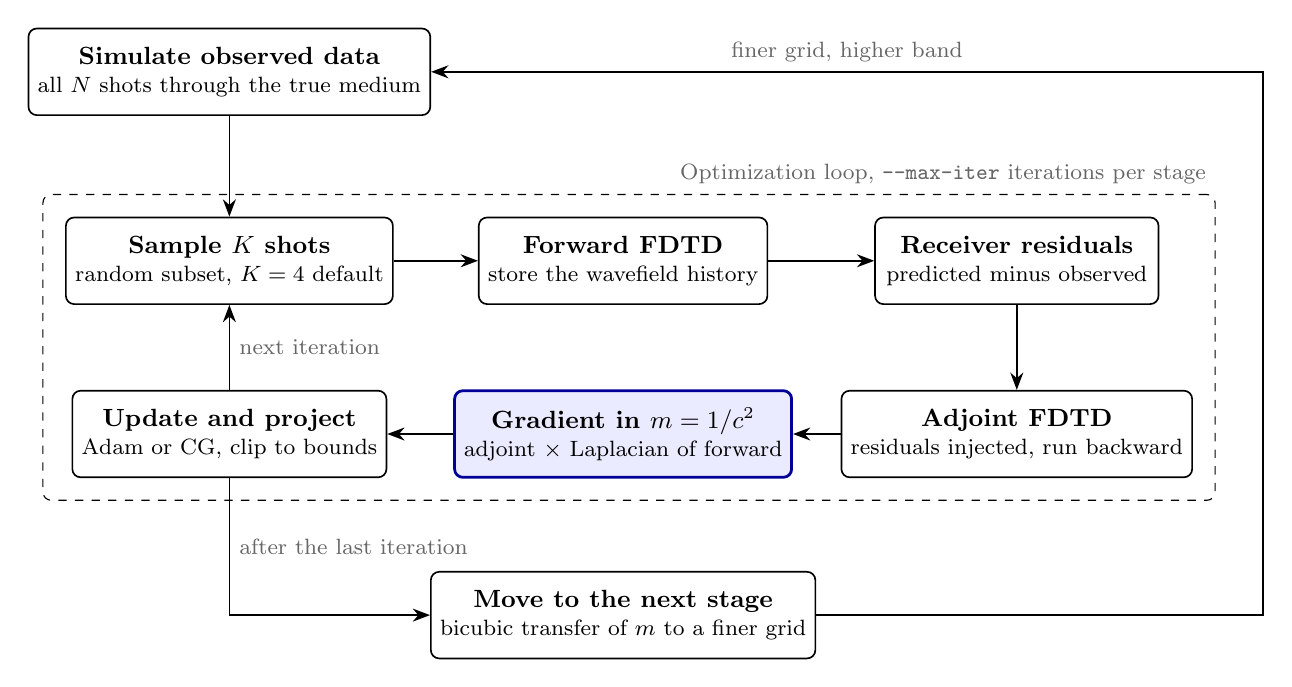
\begin{tikzpicture}[
  font=\small,
  fwbox/.style={draw, rounded corners=3pt, align=center, minimum width=3.6cm,
               minimum height=1.1cm, line width=0.6pt},
  key/.style={fwbox, draw=blue!60!black, fill=blue!8, line width=1pt},
  arrow/.style={-{Stealth[length=2.2mm]}, line width=0.6pt},
  note/.style={font=\footnotesize, text=black!60}
]
  \node[fwbox] (obs) at (0, 2.4) {\textbf{Simulate observed data}\\[-1pt]
    {\footnotesize all $N$ shots through the true medium}};
  \node[fwbox] (sample) at (0, 0) {\textbf{Sample $K$ shots}\\[-1pt]
    {\footnotesize random subset, $K = 4$ default}};
  \node[fwbox] (fwd) at (5, 0) {\textbf{Forward FDTD}\\[-1pt]
    {\footnotesize store the wavefield history}};
  \node[fwbox] (res) at (10, 0) {\textbf{Receiver residuals}\\[-1pt]
    {\footnotesize predicted minus observed}};
  \node[fwbox] (adj) at (10, -2.2) {\textbf{Adjoint FDTD}\\[-1pt]
    {\footnotesize residuals injected, run backward}};
  \node[key] (grad) at (5, -2.2) {\textbf{Gradient in $m = 1/c^2$}\\[-1pt]
    {\footnotesize adjoint $\times$ Laplacian of forward}};
  \node[fwbox] (upd) at (0, -2.2) {\textbf{Update and project}\\[-1pt]
    {\footnotesize Adam or CG, clip to bounds}};
  \node[fwbox] (next) at (5, -4.5) {\textbf{Move to the next stage}\\[-1pt]
    {\footnotesize bicubic transfer of $m$ to a finer grid}};

  \node[draw, dashed, rounded corners=3pt, inner sep=8pt,
        fit=(sample)(res)(adj)(upd), label={[note, anchor=south east]north east:Optimization loop, \code{-{}-max-iter} iterations per stage}] (loop) {};

  \draw[arrow] (obs) -- (sample);
  \draw[arrow] (sample) -- (fwd);
  \draw[arrow] (fwd) -- (res);
  \draw[arrow] (res) -- (adj);
  \draw[arrow] (adj) -- (grad);
  \draw[arrow] (grad) -- (upd);
  \draw[arrow] (upd.north) -- node[note, right] {next iteration} (sample.south);
  \draw[arrow] (upd.south) |- node[note, pos=0.25, right] {after the last iteration} (next.west);
  \draw[arrow] (next.east) -| ([xshift=6mm]loop.east) |- node[note, pos=0.75, above] {finer grid, higher band} (obs.east);
\end{tikzpicture}
\caption{FWI loop inside each multiscale stage. Every iteration costs one
  forward and one adjoint solve per sampled shot; the three stages repeat the
  whole loop at 25--75, 50--125 and 100--250~kHz.}
\label{fig:loop}
\end{figure}

\section{Implementation and verification}
\label{sec:verification}

The adjoint gradient matches finite differences to second order, and the cost
of one iteration is two wave solves per sampled shot plus the stored wavefield.

\begin{itemize}
  \item \textbf{Batching.} \code{TorchFDTD2DBatch} advances up to
    \code{-{}-parallel-shots} independent shots as one (batch, $n_y$, $n_x$)
    tensor; forward and adjoint passes share the same Laplacian convolution and
    Mur update. On CUDA both are compiled with
    \code{torch.compile(mode="reduce-overhead")}.
  \item \textbf{Memory.} The forward pass keeps every time step of every shot in
    the batch for the adjoint. In float32 this is
    $n_{\mathrm{steps}} \times n_y \times n_x \times 4$ bytes per shot: about
    1.3~GB for the $401^2$ phantom grid and 1.95~GB for the $401^2$ s1366
    abdomen stage (3039 steps). The batch size is therefore memory-bound on the
    final stage; the s1366 run used \code{-{}-parallel-shots 2} on a 17~GB
    machine.
  \item \textbf{Gradient check.} \code{python invert\_ring.py -{}-gradient-check
    -{}-dtype float64} compares the adjoint directional derivative
    $g \cdot \delta m$ with central differences on a $41 \times 41$ grid with a
    12~mm, 1800~m/s inclusion (Table~\ref{tab:gradcheck}).
\end{itemize}

\begin{table}[ht]
\centering
\small
\caption{Adjoint gradient check (float64, run on September 28, 2026).}
\label{tab:gradcheck}
\begin{tabular}{@{}cc@{}}
\toprule
Step $\varepsilon$ & Relative error \\
\midrule
$10^{-2}$ & $3.5\times10^{-3}$ \\
$10^{-3}$ & $3.4\times10^{-5}$ \\
$10^{-4}$ & $3.4\times10^{-7}$ \\
\bottomrule
\end{tabular}
\end{table}

The error falls $100\times$ per $10\times$ smaller step, the expected behaviour
for a correct gradient with a second-order difference; the approximate adjoint
of the Mur boundary does not show at this level. A pytest suite
(\code{tests/}) checks the neural parameterization's chain rule the same way on
ring and arc problems.

\section{Abdomen imaging results}
\label{sec:results}

Three-stage FWI of the segmentation-based s1366 abdomen fits the data better
at every stage, but the final model is no closer to the true speeds overall:
its interior RMS error is 314.7~m/s, against 293.1~m/s for the uniform
1480~m/s starting model. The bone, 1.6\% of the interior, drives this result.

\subsection{Segmentation-based abdomen (TotalSegmentator s1366)}
\label{sec:s1366}

The run used the s1366 map of Section~\ref{sec:totalseg} and the setup of
Table~\ref{tab:setup}:
\begin{verbatim}
python invert_ring.py --device cpu --ct-speed totalseg_s1366_acoustic.npz \
  --multiscale --n-elements 128 --n-shots 4 --parallel-shots 2 \
  --max-iter 50 --adam-lr 4e-9 --c-min 1400 --c-max 3900
\end{verbatim}
The full log is in \code{totalseg\_s1366\_multiscale\_log.txt}.

\begin{table}[ht]
\centering
\small
\caption{s1366 multiscale run, per stage (50 Adam iterations each; 8 CPU
  threads, float32). $J$ is computed on the 4 random shots of each iteration,
  so values are noisy and not comparable between stages.}
\label{tab:s1366}
\begin{tabular}{@{}lrrrr@{}}
\toprule
Stage & $J$ at iteration 1 & $J$ at iteration 50 & Observed data (s) & Optimization (s) \\
\midrule
$101^2$, 4.00~mm, 25--75~kHz & $2.83\times10^{4}$ & $2.40\times10^{3}$ & 15 & 72 \\
$201^2$, 1.83~mm, 50--125~kHz & $9.55\times10^{3}$ & $1.41\times10^{3}$ & 74 & 433 \\
$401^2$, 1.50~mm, 100--250~kHz & $1.50\times10^{4}$ & $8.70\times10^{3}$ & 165 & 2660 \\
\midrule
Total wall time & \multicolumn{4}{r}{3419~s (57~min)} \\
\bottomrule
\end{tabular}
\end{table}

\begin{figure}[ht]
  \centering
  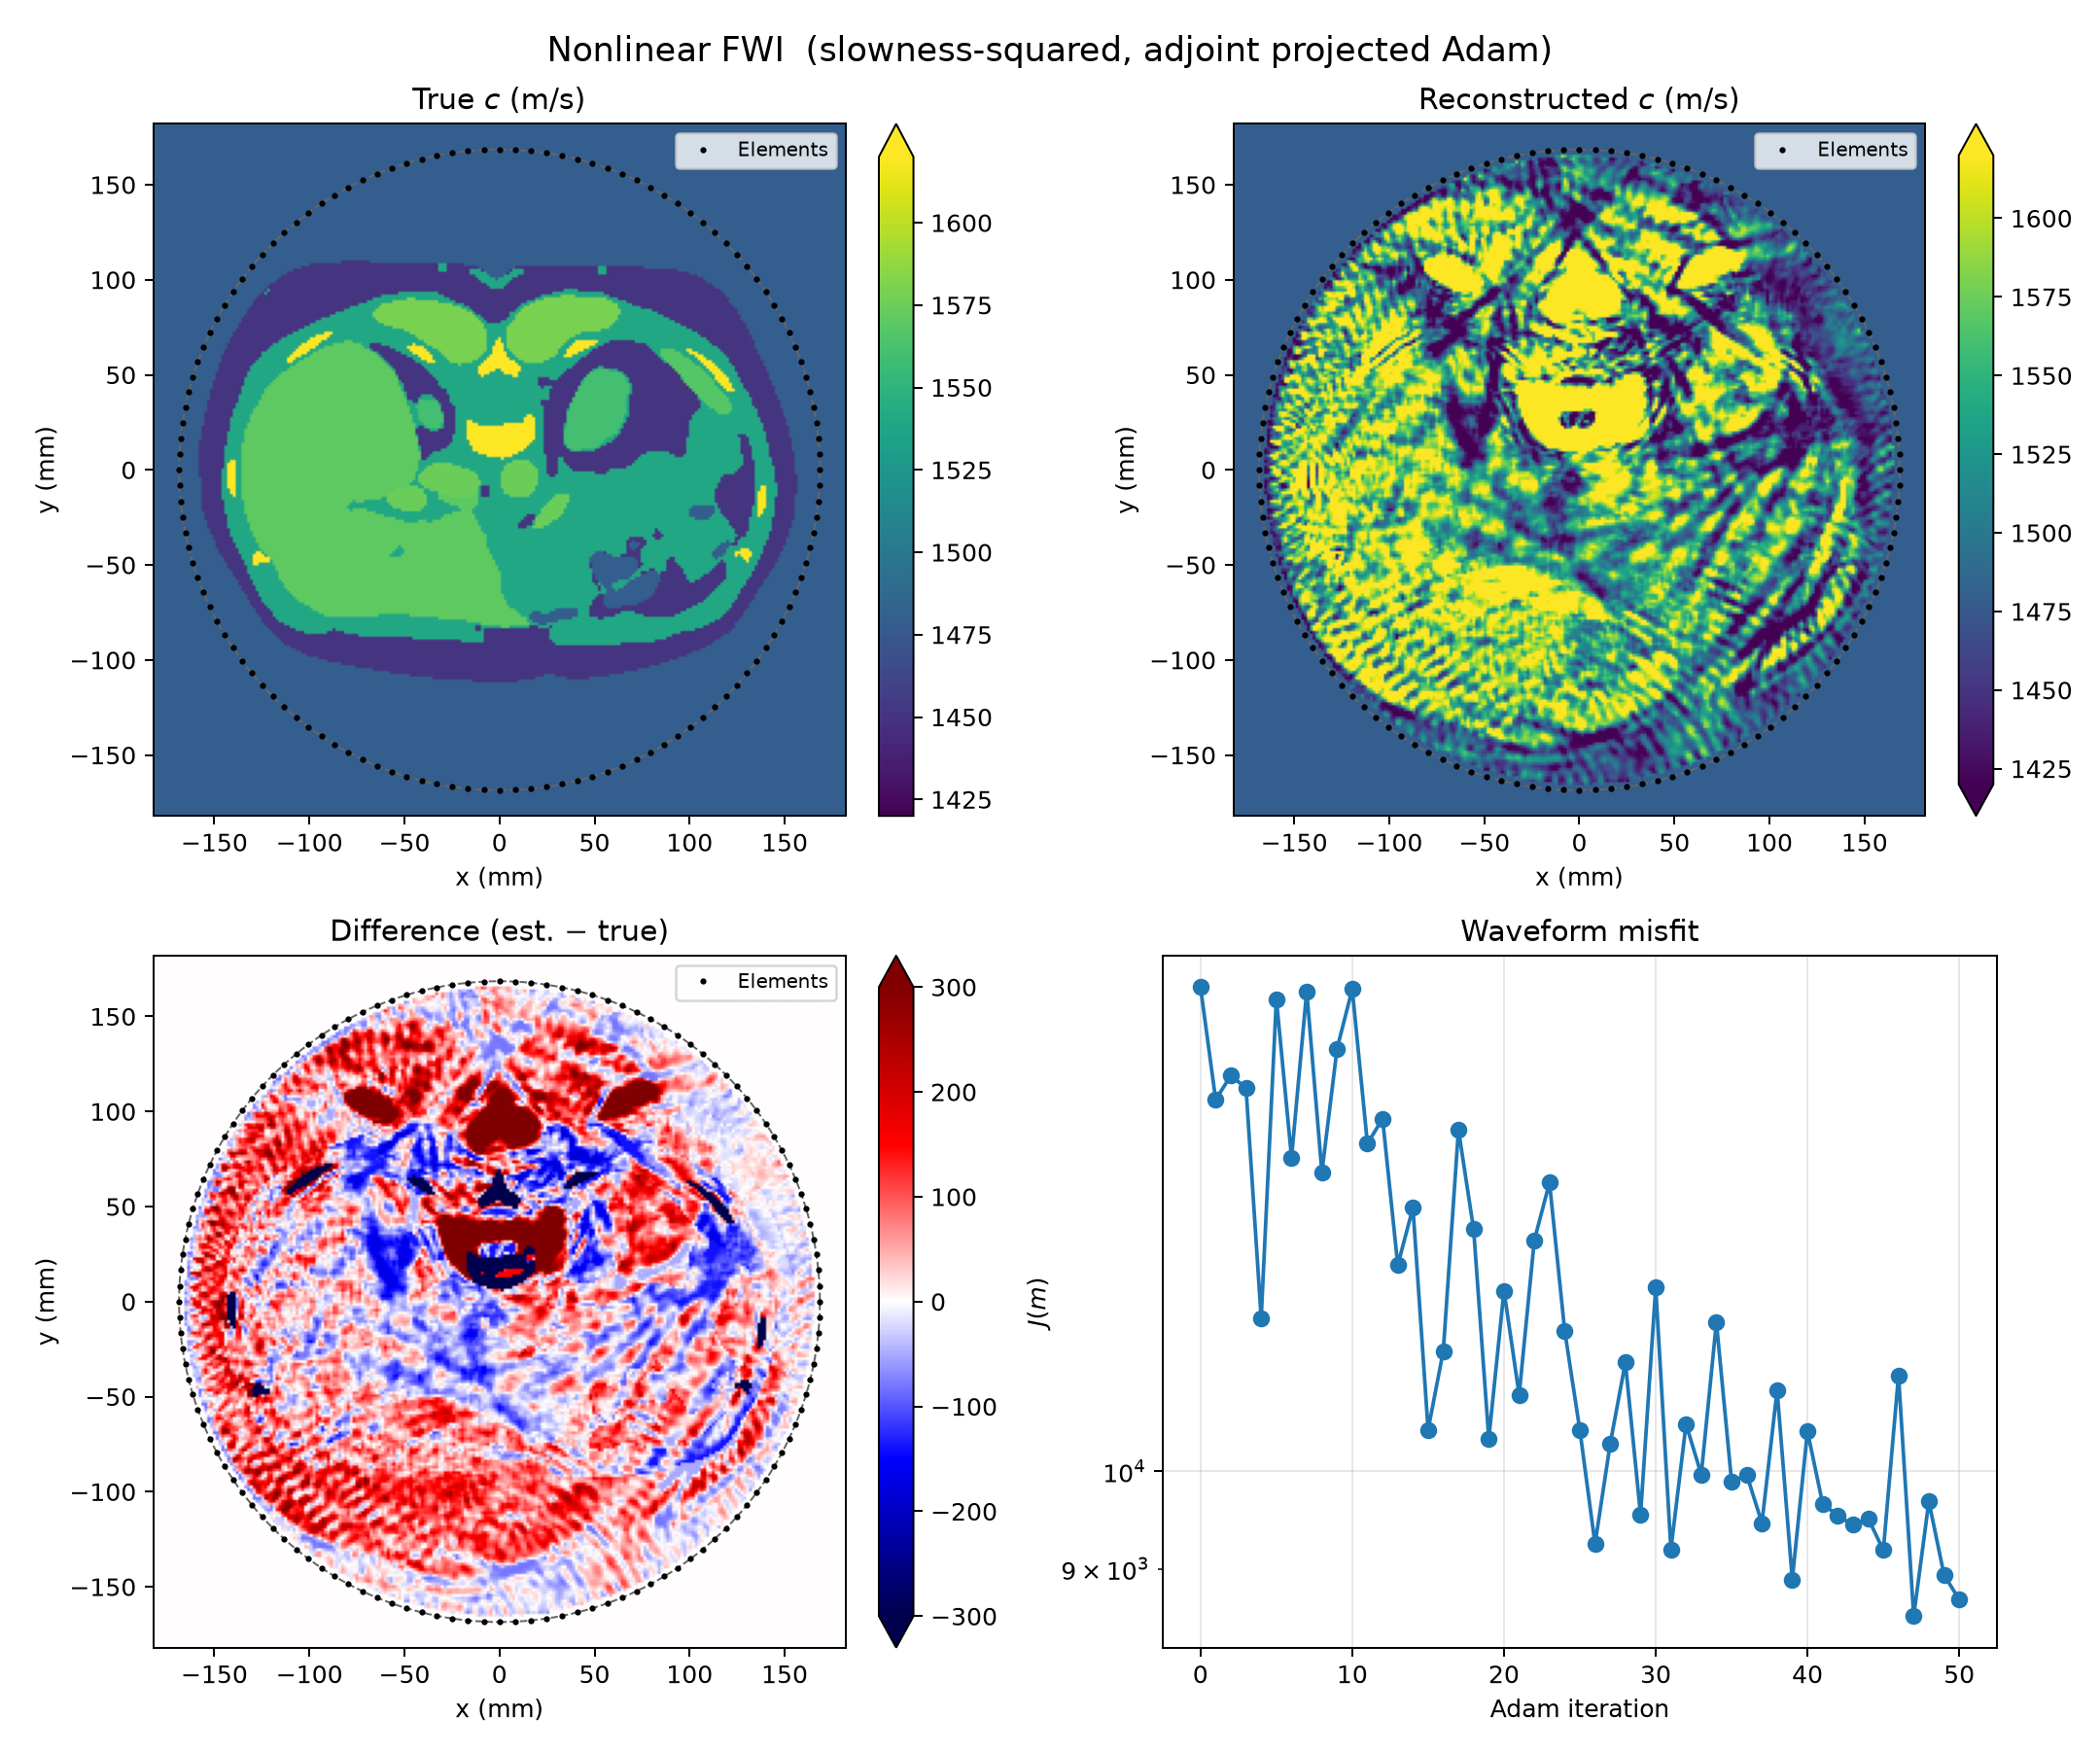
\includegraphics[width=\textwidth]{totalseg_s1366_multiscale.png}
  \caption{Multiscale FWI of the s1366 abdomen. True $c$, reconstruction after
    the $401^2$ / 100--250~kHz stage, difference, and the final-stage misfit.
    The plot's $y$ axis runs anterior (bottom) to posterior (top).}
  \label{fig:s1366}
\end{figure}

\begin{itemize}
  \item \textbf{Bone.} The vertebral body is recovered as a ring: too fast at
    its anterior rim (up to $+2000$~m/s) and still too slow inside (about
    $-2000$~m/s). The thin ribs are not recovered (blue arcs in the
    difference map).
  \item \textbf{False bone-speed patches.} Three patches reach 2500--3500~m/s
    in the posterior soft tissue near the spinous process and posterior ribs,
    where the true speed is 1450--1580~m/s.
  \item \textbf{Soft tissue.} Away from the bone the error is mostly within a
    few hundred m/s, with ring-shaped streaks from the 128-element aperture;
    organ boundaries are only faintly visible.
  \item \textbf{Convergence.} $J$ falls $12\times$ and $7\times$ in the first
    two stages but only $1.7\times$ in the last, where it stays noisy.
  \item \textbf{RMS error.} 314.7~m/s, against 293.1~m/s for the starting
    model. Without the bone pixels the starting model's error is only
    53.3~m/s, so the bone errors and the false high-speed patches dominate the
    final figure.
\end{itemize}

Compared with the KiTS-00136 run (Section~\ref{sec:kits}), the s1366 result
has twice as many elements but a coarser final grid (1.5 versus 1.01~mm,
3.9 points per wavelength). Faster bone (3750 versus 3476~m/s) and thin ribs
make the cycle skipping worse.

\subsection{Earlier experiment: KiTS-00136 with the HU-threshold model}
\label{sec:kits}

The first abdomen runs used the \code{ct\_to\_speed.py} map of C4KC-KiTS case
KiTS-00136 (categorical mapping, 1478--3476~m/s). Its stages ran at 4.63, 2.12
and 1.01~mm on 468, 425 and 406~mm fields of view, with a 194.4~mm ring of 64
elements (19~mm pitch). Three-stage FWI recovered the soft-tissue anatomy and
the outer cortex of the vertebra, but left the vertebral body hollow,
underestimated by up to about 2000~m/s.

\subsubsection{Full multiscale reconstruction}

\begin{figure}[ht]
  \centering
  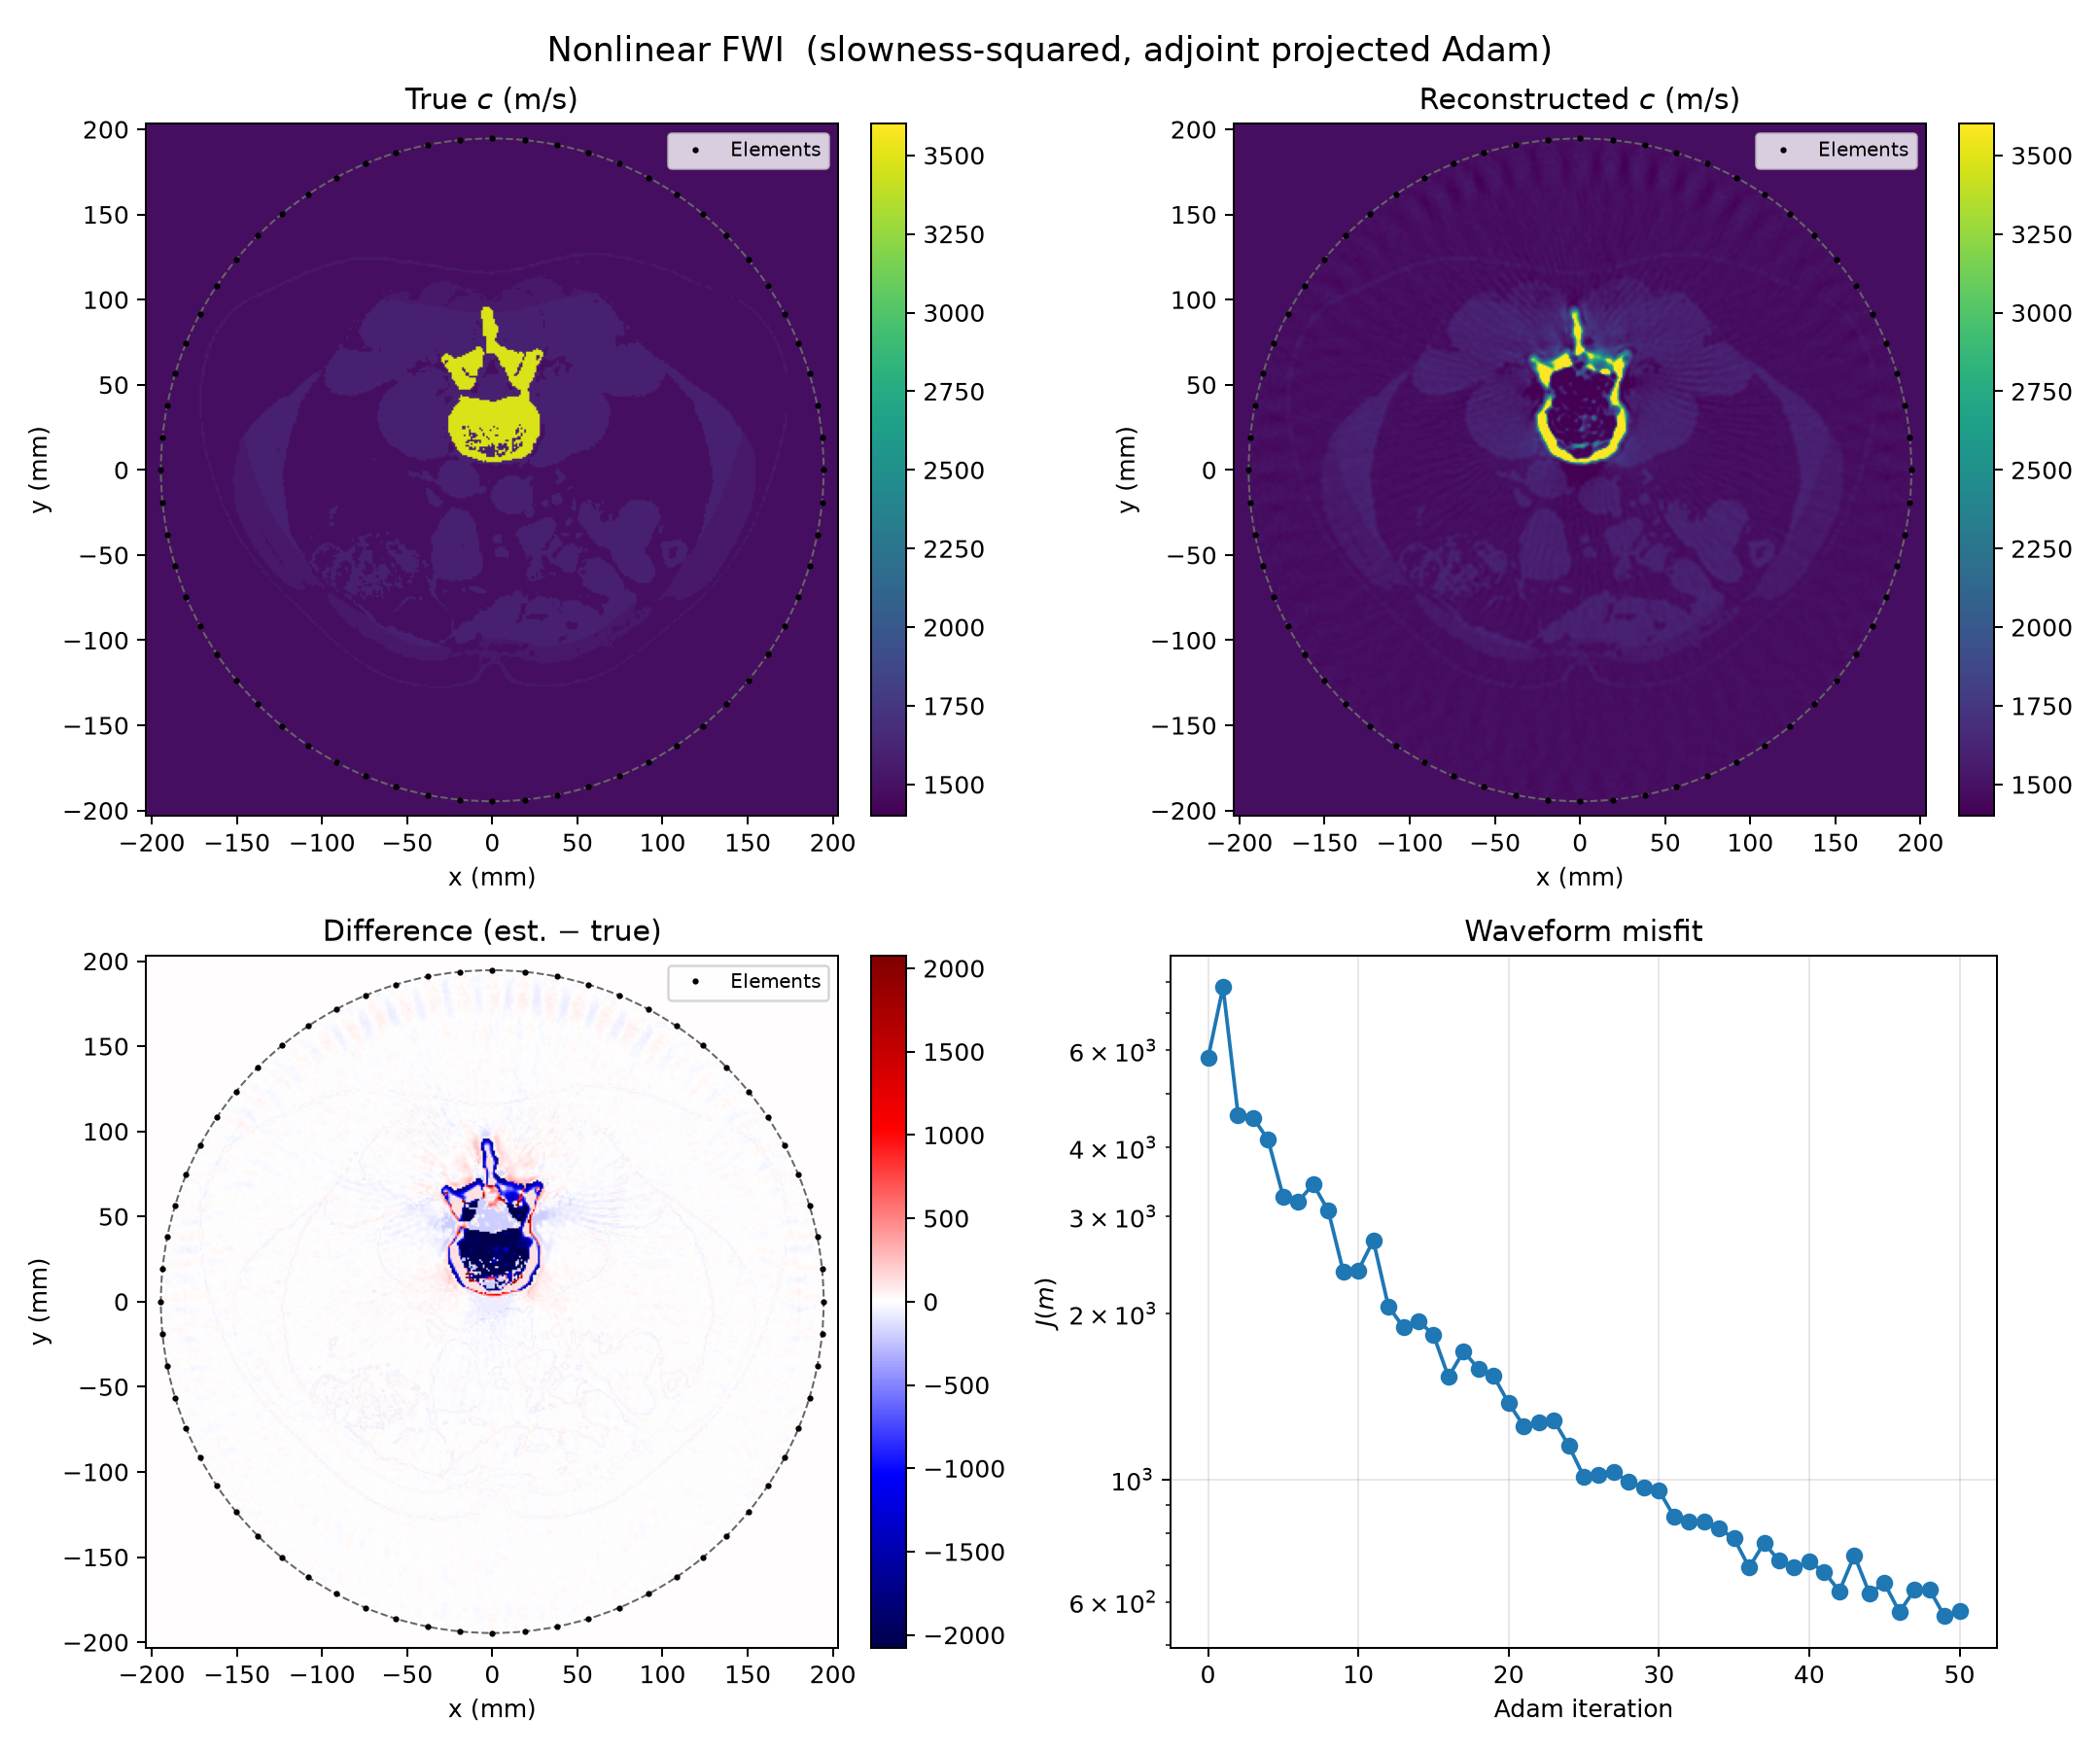
\includegraphics[width=\textwidth]{abdomenmultiscale.png}
  \caption{Multiscale FWI of the abdomen (\code{abdomenmultiscale.png},
    committed September 26, 2026). True $c$, reconstruction after the
    $401^2$ / 100--250~kHz stage, difference, and the final-stage waveform
    misfit over 50 Adam iterations.}
  \label{fig:multiscale}
\end{figure}

\begin{itemize}
  \item \textbf{Soft tissue.} Organ boundaries, the paraspinal muscles, the
    abdominal-wall muscle and the fat layers appear in the right places with
    roughly the right speeds; the difference map is near zero across most of
    the abdomen.
  \item \textbf{Bone.} The cortical rim of the vertebral body and the posterior
    elements are recovered, partly at the full 3476~m/s. The interior of the
    vertebral body stays near the background speed, the dark region in the
    difference map.
  \item \textbf{Artifacts.} Faint radial streaks fan inward from the ring. With
    64 elements the pitch is about 19~mm, several wavelengths at
    100--250~kHz, so the source and receiver sampling is sparse at the finest
    stage.
  \item \textbf{Convergence.} In the final stage $J$ falls from about
    $5.9\times10^{3}$ to about $5.8\times10^{2}$ (roughly $10\times$, read from
    the plot), with a rise after the first step and the noise expected from
    random shot sub-sampling.
\end{itemize}

The command line for this run was not saved. Its setup is inferred from the figure (ring radius, 64 plotted
elements, 50 Adam iterations per stage) and the code defaults.

\subsubsection{Coarse-stage reproduction}

To give logged numbers, the first stage was rerun on CPU on October 27, 2026
with
\begin{verbatim}
python invert_ring.py --ct-speed abdomen_acoustic.npz --coarse-only \
  --n-elements 64 --n-shots 4 --max-iter 50 --adam-lr 4e-9 \
  --c-min 1400 --c-max 3600
\end{verbatim}
The full log is in \code{abdomen\_coarse\_stage\_log.txt}.

\begin{table}[ht]
\centering
\small
\caption{Coarse-stage abdomen reproduction.}
\label{tab:coarse}
\begin{tabular}{@{}ll@{}}
\toprule
Quantity & Value \\
\midrule
Grid / band & $101 \times 101$ at 4.63~mm, 25--75~kHz \\
Time steps, $\Delta t$ & 1029, 409~ns \\
Misfit $J$, start $\to$ end & $7.35\times10^{3} \to 1.35\times10^{3}$ ($5.4\times$ lower) \\
Interior RMS error in $c$ & 298.5~m/s \\
Interior $c$ range, true & 1478--3476~m/s \\
Interior $c$ range, reconstructed & 1400--1832~m/s \\
Wall time (8 CPU threads, float32) & 71~s (observed data 2.1~s, optimization 68.6~s) \\
\bottomrule
\end{tabular}
\end{table}

\begin{figure}[ht]
  \centering
  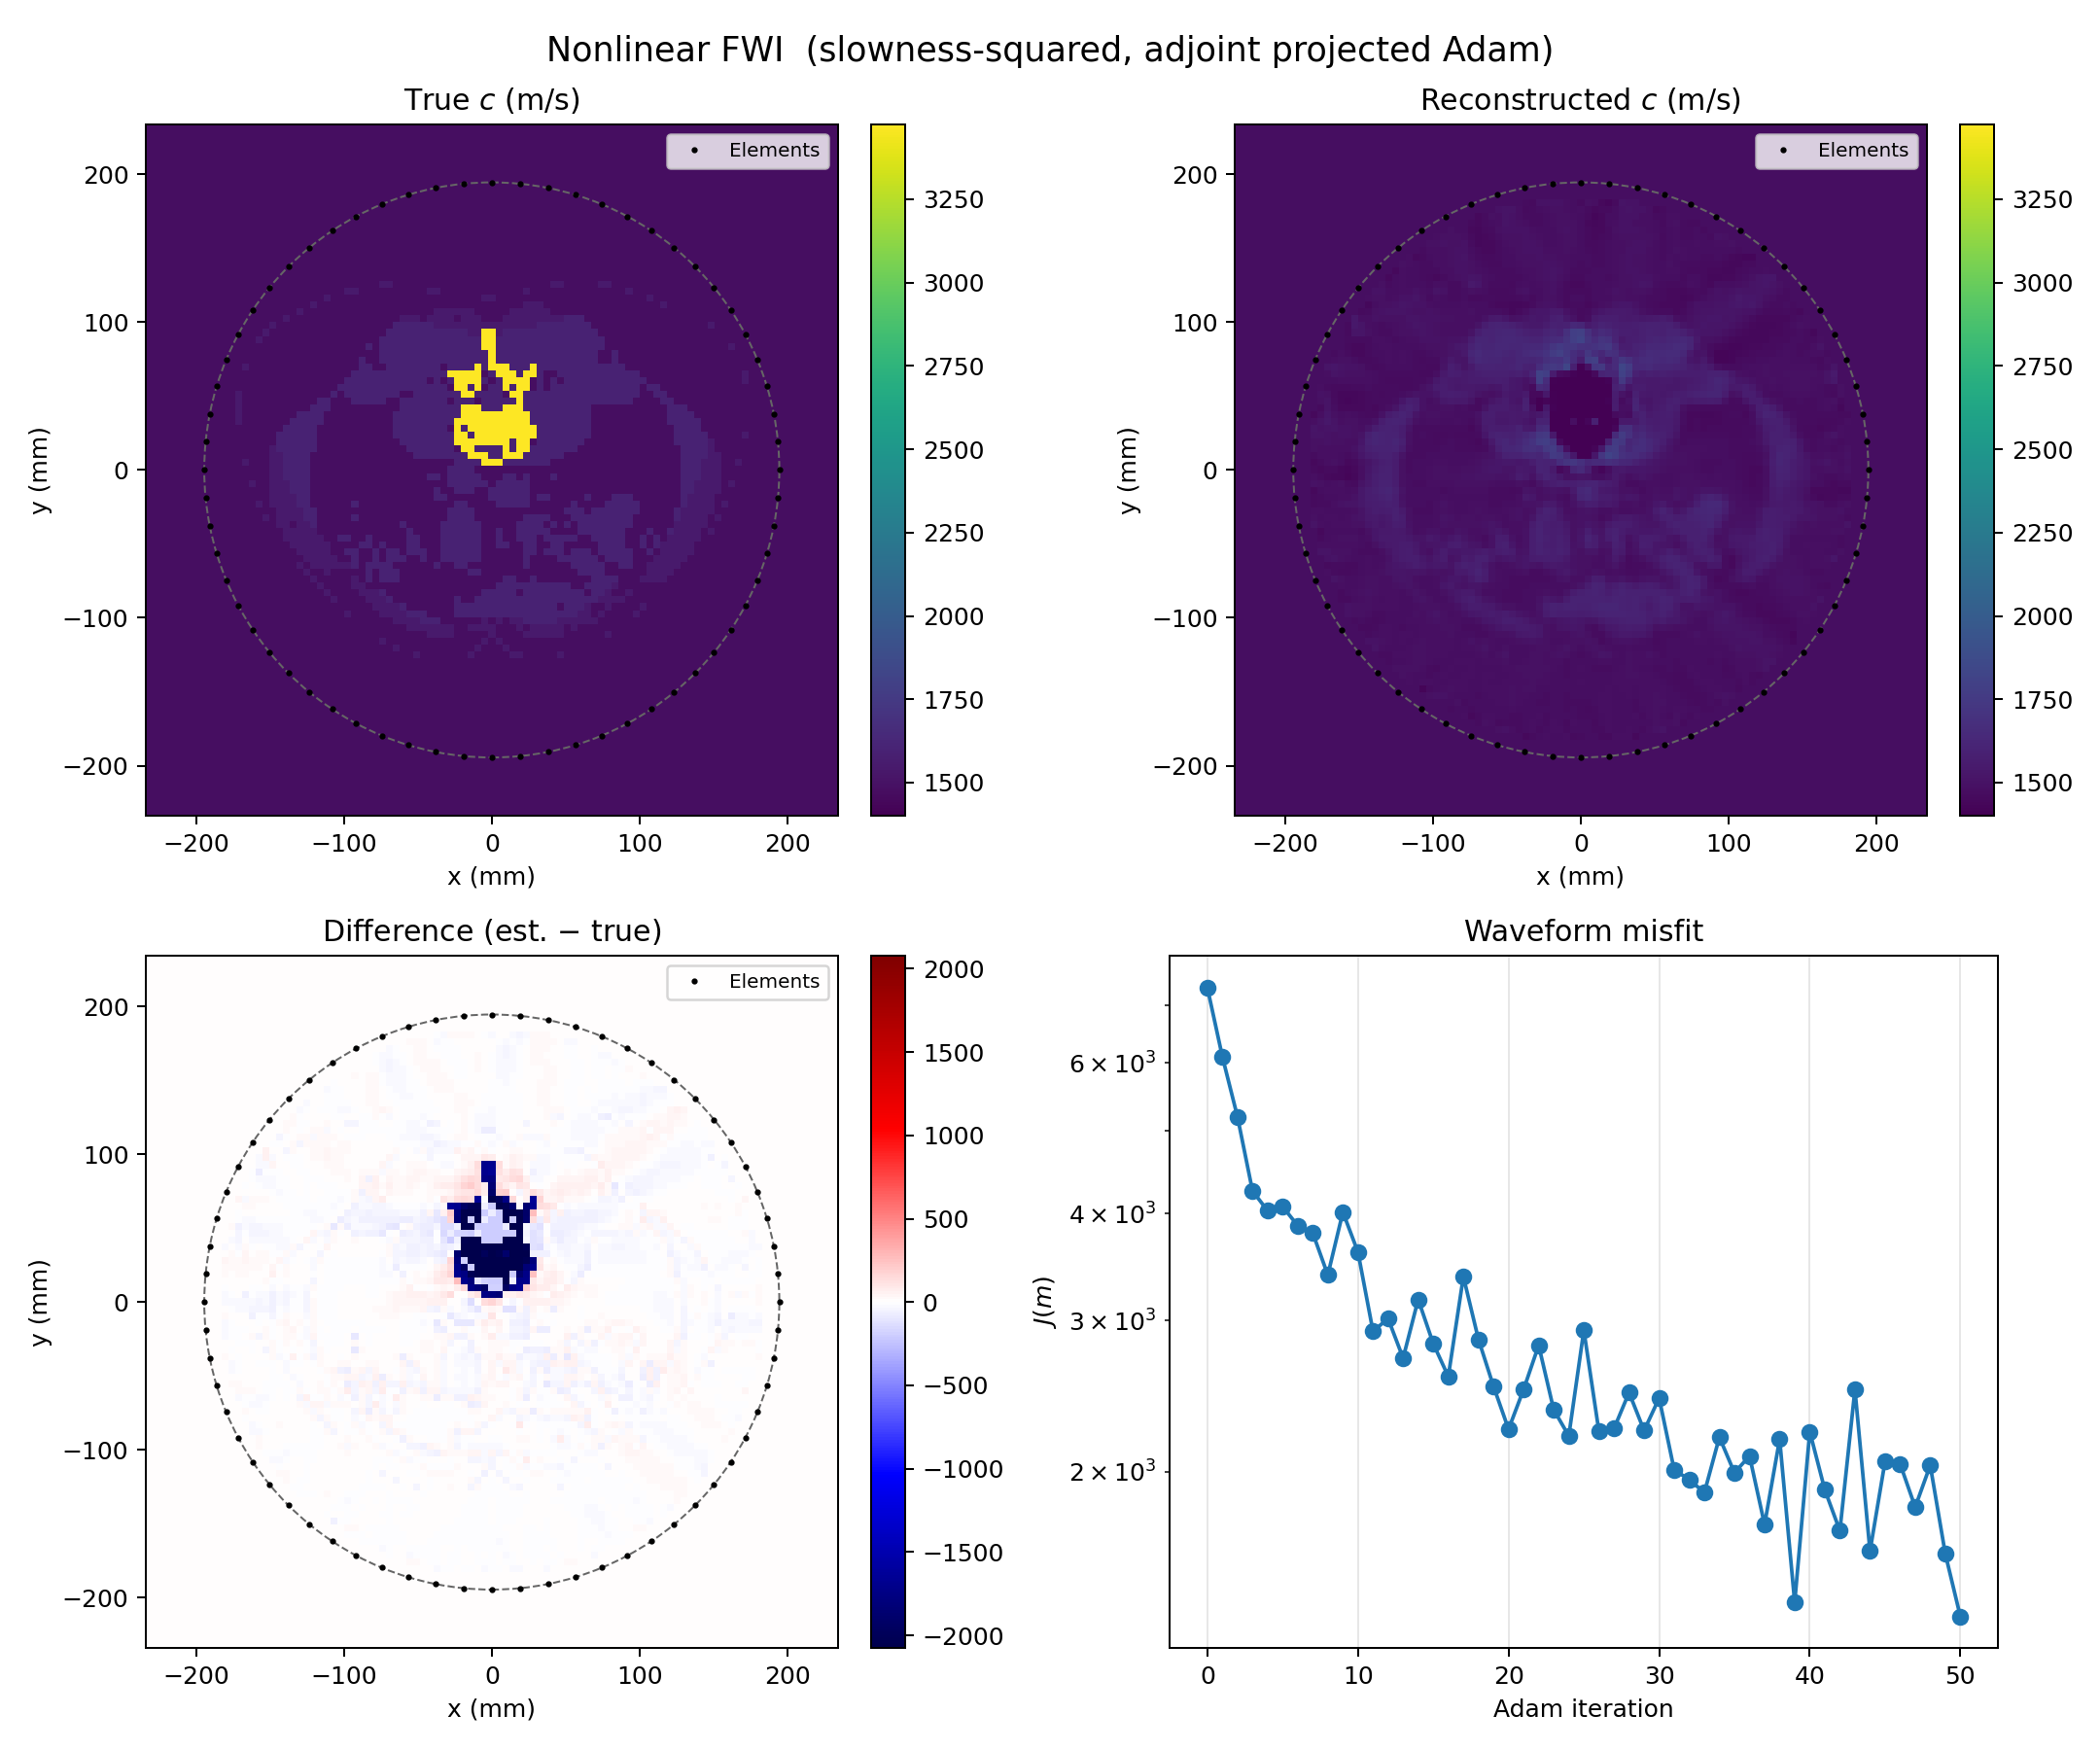
\includegraphics[width=\textwidth]{abdomen_coarse_stage.png}
  \caption{Coarse stage only ($101^2$, 25--75~kHz, 50 Adam iterations). Organ
    and muscle outlines are already visible; the vertebra region is driven down
    to the 1400~m/s lower bound.}
  \label{fig:coarse}
\end{figure}

The soft-tissue structures appear after a single coarse stage, but the vertebra
goes the wrong way: speed falls to the lower bound where it should rise to
3476~m/s. A straight path through about 40~mm of bone arrives about 15~$\mu$s
earlier than through water, more than half the 13~$\mu$s period at 75~kHz, so
the coarse data are already cycle-skipped there. The later stages start from
this hollow vertebra and only sharpen its rim, which matches
Figure~\ref{fig:multiscale}. The RMS error is dominated by the bone pixels; the
difference map is close to zero over most of the soft tissue.

\section{Limitations and next steps}

The main limits are the inverse crime, the bone, and the coarse sampling of the
abdomen setup.

\begin{itemize}
  \item \textbf{Inverse crime.} Observed and predicted data come from the same
    solver on the same grid, with no noise. Results are optimistic; data should
    be generated on a finer grid, or with an independent solver, plus noise.
  \item \textbf{Bone and cycle skipping.} The $2.5\times$ speed contrast of
    bone cycle-skips even at 25--75~kHz and, in the s1366 run, leaves the final
    RMS error above the starting model's. Options: start below 25~kHz, add a
    travel-time or envelope misfit for the first stage, begin from a
    bone-aware prior (the segmentation already marks the bone), or invert soft
    tissue only with the bone held fixed.
  \item \textbf{Grid resolution.} The abdomen stages run at about 4--6 points
    per shortest wavelength (3.9 on the s1366 final stage, limited by the
    1.5~mm CT voxels), low for a second-order scheme; numerical dispersion is
    masked only because data and model share the grid.
  \item \textbf{Element count.} 64 elements on a 194~mm ring (19~mm pitch)
    undersample the wavefield at 100--250~kHz and produce radial streaks. More
    elements, or more shots per iteration, should reduce them.
  \item \textbf{Physics.} Constant density, no attenuation and no shear waves.
    Bone and gas are only approximated by a scalar acoustic model. The
    density and attenuation maps written by \code{totalseg\_to\_speed.py} are
    not yet used by the solvers.
  \item \textbf{Reproducibility.} The KiTS-00136 multiscale run's settings
    were not logged; the s1366 run's command and log are saved alongside its
    figure.
  \item \textbf{Memory.} Storing the full forward wavefield (about 3~GB per shot
    on the $401^2$ abdomen stage) caps the batch size; checkpointing would lift
    this.
\end{itemize}

\section*{Sources}

\begin{itemize}
  \item Repository
    \href{https://github.com/scjoshi/SoundWaveSimulation}{scjoshi/SoundWaveSimulation}:
    \code{invert\_ring.py}, \code{fdtd2d/torch\_backend.py},
    \code{fdtd2d/inversion/} (CG, misfit, medium), \code{fdtd2d/ct\_medium.py},
    \code{ct\_to\_speed.py}, \code{fdtd2d/inversion/neural.py}.
  \item s1366 run: \code{totalseg\_s1366\_multiscale.png} and
    \code{totalseg\_s1366\_multiscale\_log.txt}; converter
    \code{totalseg\_to\_speed.py} and \code{abdominal\_acoustic\_parameters.csv}.
  \item Abdomen figure \code{abdomenmultiscale.png}, commit \code{2de3791}
    (September 26, 2026); CT map figure \code{abdomen\_acoustic.png}.
  \item CT slice: \code{ct-abdomen-c4kc-kits-instance.dcm}, C4KC-KiTS
    collection, The Cancer Imaging Archive.
  \item Coarse-stage reproduction: run on October 27, 2026; gradient check: run
    on September 28, 2026 (both CPU, PyTorch 2.6).
\end{itemize}

\begin{thebibliography}{9}
\bibitem{duck1990}
F.~A. Duck, \emph{Physical Properties of Tissue: A Comprehensive Reference
Book}. London: Academic Press, 1990.

\bibitem{szabo}
T.~L. Szabo, \emph{Diagnostic Ultrasound Imaging: Inside Out}, 2nd~ed.
Elsevier Academic Press, 2014.

\bibitem{mast2000}
T.~D. Mast, ``Empirical relationships between acoustic parameters in human soft
tissues,'' \emph{Acoustics Research Letters Online}, vol.~1, no.~2,
pp.~37--42, 2000.

\bibitem{wasserthal2023}
J.~Wasserthal \emph{et al.},
``TotalSegmentator: robust segmentation of 104 anatomic structures in CT
images,'' \emph{Radiology: Artificial Intelligence}, vol.~5, no.~5, e230024, 2023.

\bibitem{totalseg_data}
J.~Wasserthal, ``Small subset of TotalSegmentator Dataset,'' version 2.0.1,
Zenodo, 2023, \url{https://zenodo.org/records/10047263} (CC BY 4.0).

\bibitem{culjat2010}
M.~O. Culjat, D.~Goldenberg, P.~Tewari, and R.~S. Singh,
``A review of tissue substitutes for ultrasound imaging,''
\emph{Ultrasound in Medicine \& Biology}, vol.~36, no.~6, pp.~861--873, 2010.
\end{thebibliography}

\end{document}
